\documentclass[./main.tex]{subfiles}
\graphicspath{{\subfix{./images/}}}

\begin{document}

\subsection{Re-evaluating Arrays as a data structure}

In order to understand the properties, advantages and disadvantages of linked lists, we must re-evaluate how arrays work. Take this array
in Java as an example:

\begin{minted}{java}
int[] nums = {3, 4, 5, 6};
\end{minted}

the array \emph{\texttt{nums}} stores multiple numbers in the same variable by placing them next to each other in memory. For example:

\begin{figure}[htbp]
    \centering
    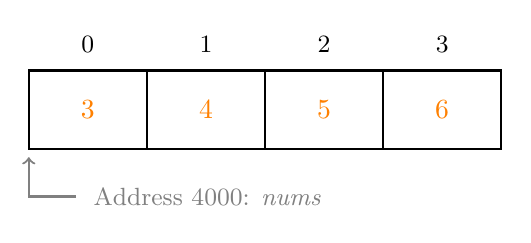
\begin{tikzpicture}
        \foreach \i/\v in {0/3,1/4,2/5,3/6} {
            \pgfmathsetmacro\x{\i*1.5}
            \draw[thick] (\x,0) rectangle (\x+1.5,1);
            \node[anchor=south] at (\x+0.75,1.1) {\mono \small \i};
            \node[orange] at (\x+0.75, 0.5) {\monobold{\v}};
        }
        \draw[gray,thick,->] (0.6, -0.6) -| (0,-0.1);
        \node[gray,anchor=west] at (0.7, -0.6) {\mono \small Address 4000: \emph{nums}};
    \end{tikzpicture}
    \caption{the array in the above code block in memory}
    \label{fig:array}
\end{figure}

Since the items of the array are stored next to each other in memory, accessing specific indices\footnote{indexes} is simple.
Let us assume that each number in the array is a Java {\mono int} which is a 4 byte wide/32 bit wide integer.
In memory, the array would look as such:

\begin{figure}[htbp]
    \centering
    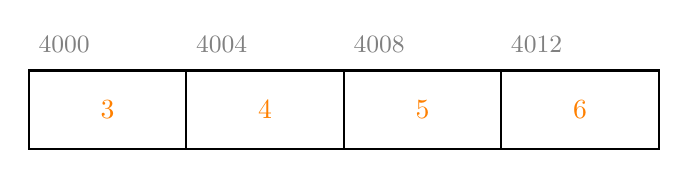
\begin{tikzpicture}
        \foreach \i/\v/\addr in {0/3/4000,1/4/4004,2/5/4008,3/6/4012} {
            \pgfmathsetmacro\x{\i*2}
            \draw[thick] (\x,0) rectangle (\x+2,1);
            \node[orange] at (\x+1, 0.5) {\monobold{\v}};
            \node[gray,anchor=south west] at (\x,1.1) {\mono \small \addr};
        }
    \end{tikzpicture}
    \caption{the addresses where the integers begin are now labeled.}
    \label{fig:array-memory}
\end{figure}

The locations of the integers in memory follow a \emph{predictable} pattern. Therefore, it is easy to access arbitrary
array indices by simply performing a math calculation. You can simply repeatedly add 4 until you get the nth index you desire,
and add it to where the array begins in memory\footnote{the actual formula is an exercise for the reader}, and ask the computer
to access that index \emph{very cheaply}. One index, one calculation.

The issue with arrays, are that in order to insert new elements, you must create entirely new memory.
This is because all arrays have a fixed and predetermined size. There might be memory after or before the array that is already
in use, which cannot be moved.

Therefore, one could produce a new array and copy all the data from the old memory to it.

\newpage

\begin{figure}[htbp]
    \centering
    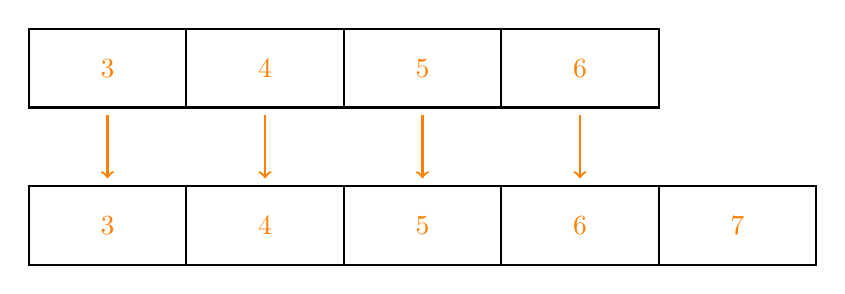
\begin{tikzpicture}
        \foreach \i/\v in {0/3,1/4,2/5,3/6} {
            \pgfmathsetmacro\x{\i*2}
            \draw[thick] (\x,2) rectangle (\x+2,3);
            \node[orange] at (\x+1, 2.5) {\monobold{\v}};
            \draw[thick,orange,->] (\x+1,1.9) -- (\x+1,1.1);
        }
        \foreach \i/\v in {0/3,1/4,2/5,3/6,4/7} {
            \pgfmathsetmacro\x{\i*2}
            \draw[thick] (\x,0) rectangle (\x+2,1);
            \node[orange] at (\x+1, 0.5) {\monobold{\v}};
        }
    \end{tikzpicture}
    \caption{"extending" the memory requires one to make a new array and copy all elements to it.}
    \label{fig:array-extend}
\end{figure}

where 7 is the new item to be added.

In Java, this looks as such:

\begin{minted}{java}
int old[4] = {3, 4, 5, 6};
int extended[5] = new int[5];

for (int i = 0; i < old.length; i++) {
    extended[i] = old[i];
}

// we now have space to put the 7 
extended[4] = 7;
\end{minted}

However, assuming if we had 1000 elements, if we wanted to add a 1001st element, that would require copying 1000 items in memory, and having 2001 items worth of space reserved in memory until the copy is finished, at which point, Java will automatically clean up the 1000 items.

Linked lists help us solve this problem.

\subsection{Linked Lists}

Similar to arrays, linked lists allow you to store many pieces of data in a given order in one collection/group. Instead of storing items in
a continuous chunk of memory that cannot grow or shrink, Linked Lists store data as individual data points, called nodes. 
Not only do these nodes store the data itself, they also store the location of where the next item in the Linked List is.

The overall intuition is, that the ordering of the list is actually independent of the order of the items in memory.
Unlike arrays, linked lists do not assume that your items are always next to each other.
This lets you create new items and add them to the list without worrying about not having enough space. 
Conceptually, they look like this:

\begin{figure}[htbp]
    \centering
    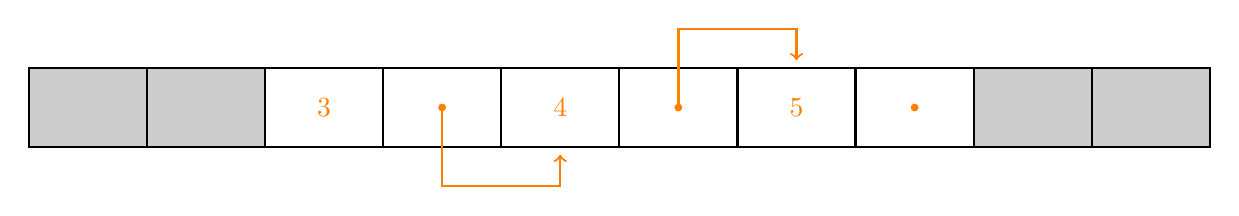
\begin{tikzpicture}
        % boxes
        \pgfmathsetmacro\w{1.5}
        \foreach \i in {0,1,2,3,4,5,6,7,8,9} {
            \pgfmathsetmacro\x{\i*\w}
            \pgfmathparse{(\i <= 1) || ((\i >= 8) && (\i <= 9))}
            \ifnum\pgfmathresult = 1 
                \draw[thick, fill=gray!40] (\x,0) rectangle (\x+\w,1);
            \else
                \draw[thick] (\x,0) rectangle (\x+\w,1);
            \fi
        }

        % numbers and dots
        \pgfmathparse{(2*\w)+(\w/2)}
        \node[orange] at (\pgfmathresult,0.5) {\monobold 3};
        \pgfmathparse{(3*\w)+(\w/2)}
        \fill[orange] (\pgfmathresult,0.5) circle (0.05);
        \pgfmathparse{(4*\w)+(\w/2)}
        \node[orange] at (\pgfmathresult,0.5) {\monobold 4};
        \pgfmathparse{(5*\w)+(\w/2)}
        \fill[orange] (\pgfmathresult,0.5) circle (0.05);
        \pgfmathparse{(6*\w)+(\w/2)}
        \node[orange] at (\pgfmathresult,0.5) {\monobold 5};
        \pgfmathparse{(7*\w)+(\w/2)}
        \fill[orange] (\pgfmathresult,0.5) circle (0.05);

        % arrows
        \pgfmathsetmacro{\beginx}{(3*\w)+(\w/2)}
        \pgfmathsetmacro{\endx}{(4*\w)+(\w/2)}
        \draw[thick,orange,->] (\beginx,0.5) -- (\beginx,-0.5) -- (\endx,-0.5) -- (\endx,-0.1);

        \pgfmathsetmacro{\beginx}{(5*\w)+(\w/2)}
        \pgfmathsetmacro{\endx}{(6*\w)+(\w/2)}
        \draw[thick,orange,->] (\beginx,0.5) -- (\beginx,1.5) -- (\endx,1.5) -- (\endx,1.1);
    \end{tikzpicture}
    \caption{Linked lists, in memory. Gray represents used memory}
    \label{fig:contiguous-ll}
\end{figure}

where each pair of boxes (number and dot with an arrow) is called a Node. For now, \emph{simply assume that nodes are just another data type, which can be the type of a variable}.

Let us assume that each node is a variable\footnote{Yes, variables \emph{can} also be stored next to each other in memory! If you declare two integers, one after another in code, they will be placed next to each other in memory, as that is simply the most efficient.}, if we create 3 nodes with the numbers {\mono 3, 4, 5}, they will be next to each other in memory. However, suppose your program runs for a while, and more memory is used by variables, function parameters, and whatnot. If you wanted to add a new item to the linked list, you would not need to reallocate anything, instead, you can just \emph{create another node somewhere else, and point the dot on the node that stores 5 to the new one.}

\begin{figure}[htbp]
    \centering
    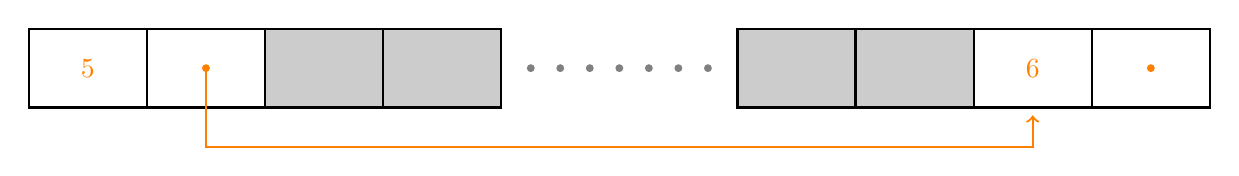
\begin{tikzpicture}
        % boxes
        \pgfmathsetmacro\w{1.5}
        % skip 4 and 5 for ellipses
        \foreach \i in {0,1,2,3,6,7,8,9} {
            \pgfmathsetmacro\x{\i*\w}
            \pgfmathparse{((\i >= 2) && (\i <= 7))}
            \ifnum\pgfmathresult = 1 
                \draw[thick, fill=gray!40] (\x,0) rectangle (\x+\w,1);
            \else
                \draw[thick] (\x,0) rectangle (\x+\w,1);
            \fi
        }

        % dots
        \foreach \i in {0,1,2,3,4,5,6} {
            \pgfmathsetmacro{\spacing}{0.25}
            \pgfmathsetmacro{\x}{3.25+(\i*\spacing)}
            \pgfmathparse{(\x*\w)+(\w/1)}
            \fill[gray] (\pgfmathresult,0.5) circle (0.05);
        }

        % data
        \pgfmathparse{(0*\w)+(\w/2)}
        \node[orange] at (\pgfmathresult,0.5) {\monobold 5};
        \pgfmathparse{(1*\w)+(\w/2)}
        \fill[orange] (\pgfmathresult,0.5) circle (0.05);

        \pgfmathparse{(8*\w)+(\w/2)}
        \node[orange] at (\pgfmathresult,0.5) {\monobold 6};
        \pgfmathparse{(9*\w)+(\w/2)}
        \fill[orange] (\pgfmathresult,0.5) circle (0.05);

        % arrows
        \pgfmathsetmacro{\beginx}{(1*\w)+(\w/2)}
        \pgfmathsetmacro{\endx}{(8*\w)+(\w/2)}
        \draw[thick,orange,->] (\beginx,0.5) -- (\beginx,-0.5) -- (\endx,-0.5) -- (\endx,-0.1);
    \end{tikzpicture}
    \caption{The gray dots represent a long section of used memory.}
    \label{fig:ll-append}
\end{figure}

This idea of the link between nodes forming the order of the list is what makes a linked list...linked. The arrows themselves are actually
\emph{pointers}, meaning that the arrows actually simply store the memory address of the beginning of the next node.

The code for a node storing a single integer each may look as such:

\begin{minted}{java}
// in Node.java
public class Node {
    // for convenience, we make these fields public
    public int data;
    public Node next;

    Node(int data) { 
        this.data = data
    }
}
\end{minted}

\subsubsection{The Difference between a Linked List and a Node}

This is a thing that many students get wrong. Linked lists are made up of Nodes. A node is simply a class with any data in it, with some sort of
{\mono next} field that refers to any given "next" node. The existence of this next field lets you store the next node in the list, and a chain
of these nodes that refer one after another is a linked list.

\subsubsection{Creating a Linked List Manually}

\subsubsection{Converting an Array to a Linked List}

\subsubsection{Iterating through a Linked List}

\subsubsection{Adding Nodes to the End of a Linked List (Appending)}

\subsubsection{Removing Nodes to the End of a Linked List}

\subsubsection{Inserting an Item at a Position in a Linked List}

\subsubsection{Removing an Item at a Position in a Linked List}


Note that linked lists do not necessarily only need to store one piece of data per node. \emph{What makes a linked list special, is that each item
(or node) only needs to store a reference to the next node for it to be a linked list}. For example, this is also a valid linked list node:


\subsubsection{Easy Questions}

\begin{enumerate}
    \item Assume a 
\end{enumerate}


\end{document}
